\chapter{Cálculo de los PDL}

\section{Revisión de literatura}
Después de revisar la literatura, encontramos que
otros autores ya han considerado polinomios discretos ortogonales
antes, principalmente en áreas de ingeniería.
Los libros y artículos más relevantes
que encontramos son
\cite{Neuman}, \cite{papel}, \cite{george},
\cite{himmelblau}, 
y \cite{rabin}. 


\subsection{Uso de polinomios discretos en problemas de ajuste de datos}
Toda la literatura citada al inicio introduce
la noción de ``polinomios discretos ortogonales''
con una misma motivación; facilitar la resolución
de problemas de ajuste de datos basados en mínimos cuadrados.

Vamos a esbozar las ideas explicadas en
\cite{george} en esta dirección. Usamos
para esto la notación empleada
en el artículo. \\

El problema central que se desea resolver es
el siguiente:
fijada una familia de polinomios
$\{ p_{i}(x) \}_{i= 0}^{k}$ tales que
\begin{equation}
\label{ec: george 14}
\partial (p_{i}) = i \hspace{0.2cm}
\textit{para toda } \hspace{0.1cm} 0 \leq i \leq k
\end{equation}
y
dados $m$ puntos de observaciones
\[
(x_{1}, f_{1}), \ldots , (x_{m}, f_{m}),
\]
con los $x_{i}$ distintos entre sí y 
\begin{equation}
\label{eq0: 7May}
k+1 < m, 
\end{equation}
se desea encontrar
\sidenote{Como se explica en el artículo \cite{george},
se pide la condición \eqref{ec: george 14}
para que cualquier polinomio de grado a lo más $k$
pueda
representarse como combinación lineal de los polinomios $p_{i}$.}
constantes $s_{i}^{(k)}$,
con $0 \leq i \leq k$, tales que 
el polinomio definido como
\[
y_{k}(x) = s_{0}^{(k)} p_{0}(x) + \ldots +  
s_{k}^{(k)} p_{k}(x) 
\]
sea tal que 
la función de $k+1$ variables

\begin{align}
\label{ec: george 16}
\Phi(s_{0}^{(k)}, \cdots, s_{k}^{(k)})
:= & \suma{\mu = 1}{m}{(f_{\mu} - \suma{h=0}{k}{
s_{h}^{(k)} p_{h}(x_{\mu})})^{2}} \nonumber \\
= &  \suma{\mu = 1}{m}{(f_{\mu} -  y_{k}(x_{\mu}) )^{2}}
\end{align}
alcance su mínimo para esta elección de constantes
$s_{i}^{(k)}$.

\begin{figure}[H]
	\sidecaption{
	El problema consiste entonces en buscar 
	a un polinomio $y_{k}(x)$ de grado a lo más $k$
	o, equivalentemente, determinar a las constantes
	$s_{0}^{(k)}$, de tal forma que la suma de los cuadrados
	de las diferencias entre 1. las mediciones reales
	$f_{\mu}$ y 2. los valores $y_{k}(x_{\mu})$ dados por el 
	modelo polinomial sea mínima.
	\label{fig: fitting_problem}
	}
	\centering
	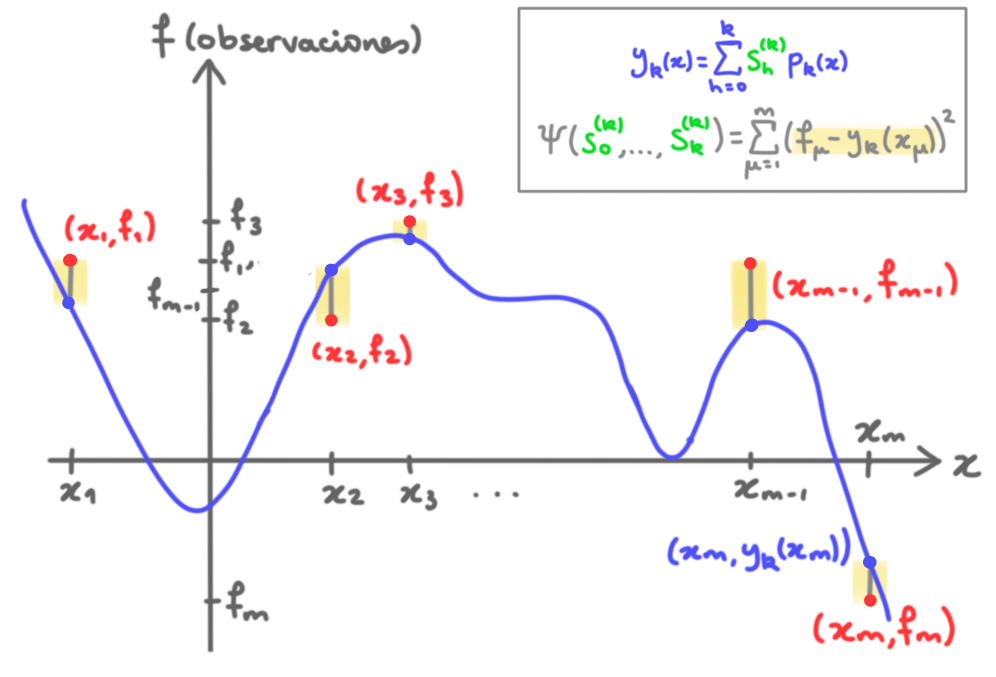
\includegraphics[scale = 1.4]{fitting_problem} 
\end{figure}	


Adoptando las abreviaciones
\begin{equation}
\label{eq: george 17}
w_{i j} = \suma{\mu=1}{m}{p_{i}(x_{\mu}) p_{j} (x_{\mu})}
\end{equation}
y
\begin{equation*}
w_{i} = \suma{\mu = 1}{m}{f_{\mu}p_{i}(x_{\mu})},
\end{equation*}
como se discute en \cite{george}, del usar que
el mínimo o máximo de una función de varias variables
$\Phi = \Phi(s_{0}^{(k)}, \cdots, s_{k}^{(k)})$
de clase $\cali{C}^{\infty}$
(como lo es $y_{k}$, por ser combinación lineal de polinomios)
sea tal que las derivadas parciales de la función
evaluadas en ese punto sean cero, se deduce el siguiente
sistema de ecuaciones:\sidenote{ En \cite{george} a tal sistema
se le denomina el ``sistema de ecuaciones normales del problema de 
ajuste de mínimos cuadrados''.}
\begin{align*}
\begin{cases}
w_{00}s_{0}^{(k)} + \ldots + w_{0k}s_{k}^{(k)} & = w_{0}, \\
\ldots & \ldots \\
w_{k0}s_{0}^{(k)} + \ldots + w_{kk}s_{k}^{(k)} & = w_{k}.
\end{cases}
\end{align*}

\noindent
En \cite{george} se nota que ``este sistema de ecuaciones
es muy general, ya que, para resolverlo, sólo se ha fijado la 
restricción de grados
\eqref{ec: george 14} en los polinomios $p_{i}$; para poder
resolver con relativa facilidad el sistema
de ecuaciones para valores altos de $k$, es suficiente
que los elementos $w_{i,j}$ con $i \neq j$
(i.e. los coeficientes no pertenecientes a la 
diagonal) sean, en comparación a los coeficientes diagonales
$w_{ii}$, pequeños. En la práctica, esto suele conseguirse 
seleccionando polinomios $p_{i}(x)$ que sean ortogonales
respecto a una distribución''.
Enseguida se nota que, pidiendo no sólo 
la restricción de grados \eqref{ec: george 14}, sino también
el que
\begin{equation}
\label{ec: george 19}
\forall i \neq j: \hspace{0.2cm}
w_{ij} = \suma{\mu=1}{m}{p_{i}(x_{\mu}) p_{j} (x_{\mu})} = 0,
\end{equation}
hecho que es descrito como el 
\textbf{``pedir que los polinomios $p_{i}(x)$
sean mutuamente ortogonales sobre el conjunto de puntos
$x_{1}, \cdots, x_{m}$''}, permite reescribir el sistema de ecuaciones 
normales como 
\begin{align*}
\begin{cases}
w_{00}s_{0}^{(k)} \ldots & = w_{0}, \\
\ldots & \ldots \\
 \ldots  w_{kk}s_{k}^{(k)} & = w_{k},
\end{cases}
\end{align*}
luego, resolverlo se reduce a calcular $k$ divisiones. 

\begin{nota}
Lo único que debe comprobarse para asegurarse de que 
este último sencillo sistema tiene solución
es que ninguno de los coeficientes $w_{ii}$ es cero;
usando la expresión \eqref{eq: george 17}, vemos 
que 
$w_{ii}$ es cero si y sólo si 
para toda $1 \leq \mu \leq m $ ocurre que
$p_{i}(x_{\mu})$. Como, según la condición 
\eqref{ec: george 14}, el grado de
$p_{i}$ es $i \leq k < m$
(c.f. \eqref{eq0: 7May}), 
es consecuencia del teorema fundamental del
álgebra 
(c.f. proposición \ref{prop: cita TFA})
el que no pueda ocurrir que todo 
$x_{\mu}$ sea raíz de $p$, luego, aseguramos
que para toda $i$ se tiene que $w_{ii} \neq 0$.
\end{nota}

La situación aquí descrita ilustra perfectamente 
por qué en la práctica es tan útil considerar
colecciones de polinomios que cumplan una condición de 
ortogonalidad (como la propuesta en \eqref{ec: george 19})
sobre un conjunto discreto.
Las otras referencias citadas al inicio del capítulo
tiene información sobre la implementación y fórmulas
concretas de tales familias de polinomios. Nosotros nos
concentramos a estudiar en particular
la referencia \cite{Neuman}, pues en 
este estudio se recopilan fórmulas que nosotros usaremos
para derivar expresiones para los
polinomios discretos de Legendre que hemos definido en el capítulo 
\ref{cap 2}.

\subsection{Polinomios discretos de Legendre en la literatura}
La fuente más completa que encontramos 
fue \cite{Neuman}, un estudio en el que se recopilan 
varias fórmulas (sin demostración) concernientes a polinomios
ortogonales de variable discreta. \\

En \cite{Neuman}, 
fijado un $N \geq 2$,
tratan con funciones $P : \{0, \ldots , N \} \rightarrow \IR$
de variable discreta, y 
se interesan en los $N+1$ ``polinomios de variable
discreta $K$''

\[
P_{m}(K, N), \hspace{0.2cm} K=0, \ldots , N,
\]
donde $m \in \{0, \ldots, N \}$ es llamado el ``grado''
del polinomio discreto, que quedan (afirman)
unívocamente determinados por las condiciones
de ortogonalidad
\begin{equation}
\suma{m=0}{n}{P_{k}(m,n) P_{l}(m,n)} =0
\hspace{0.3cm} \text{si} \hspace{0.2cm} m \neq l \tag{DLOP-1[n]} \label{eq:dlop1}
\end{equation}
y por la normalización
\begin{equation}
\text{para toda} \hspace{0.3cm} 0 \leq k \leq n, \hspace{0.3cm} P_{k}(0, n)=1.   \tag{DLOP-2[n]} \label{eq:dlop2}
\end{equation}

Para empezar a compaginar la notación
del artículo con la nuestra, 
hagamos
los cambios de variable $m=k$, $K=m$
y $N=n-1$, siendo la variable de la izquierda la empleada
originalmente en
\cite{Neuman} y la de la derecha la que usamos nosotros. \\

Pensando en los 
$n+1$ vectores de $\IR^{n+1}$ que resultan
de evaluar estas funciones discretas en su rango,
es decir, en los vectores
\begin{equation}
y_{k}:= (P_{k}(m, n))_{m=0}^{m=n}, \hspace{0.2cm}
0 \leq k \leq m,
\end{equation}
las condiciones \eqref{eq:dlop1} y \eqref{eq:dlop2}
se reinterpretan como
\begin{equation}
\{ y_{k}: \hspace{0.2cm} 0 \leq k \leq n\}
\hspace{0.3cm} \text{es una
base ortogonal de} \hspace{0.2cm} \IR^{n}
\tag{DLOP'-1[n]} \label{eq:dlop'1}
\end{equation}
y 
\begin{equation}
\text{la primera
entrada de todo} \hspace{0.2cm} y_{k} \hspace{0.2cm}
\text{es uno.} 
\tag{DLOP'-2[n]} \label{eq:dlop'2}
\end{equation}


Los autores de este estudio recopilan y derivan expresiones
analíticas (que dependen de $n$ y $k$) para estas funciones
discretas $P_{k}(\cdot ,n)$ y, del notar que los coeficientes
numéricos de estos son, salvo por posibles cambios de signo,
los de los polinomios de Legendre trasladados 
(c.f. \cite{leg})
se refieren a 
estos como \textbf{polinomios ortogonales
discretos de Legendre} (
``discrete Legendre orthogonal
polynomials'' en inglés), usando para designarlos la abreviatura
``DLOP's''. \\

Aparte de mencionar en la introducción que
``variantes de estos polinomios fueron consideradas por primera
vez por Chebyshev en 1858 y más tarde por Gram en 1915'', no se
da un marco teórico como el desarrollado por nosotros, sólo 
se dan expresiones analíticas de estos.
Los trabajos originales de Chebyshev y Gram
no están citados en las referencias del artículo, y 
nosotros no fuimos capaces de 
encontrarlos. Nos limitamos pues a usar las 
fórmulas ofrecidas en \cite{Neuman} para, a continuación,
derivar fórmulas para los polinomios discretos
de Legendre $\cali{L}^{n,k}$
como los hemos definido en el capítulo 
\ref{cap 2}.


\section{Expresión analítica de los PDL}
Fijada una dimensión $n$, planeamos usar 
las fórmulas dadas 
en ~\cite{Neuman}
para establecer expresiones analíticas
de los vectores de nuestra base $\cali{L}^{n}$; queremos,
pues, a partir de las expresiones dadas de los
elementos de la base
\begin{equation}
\label{eq: base DLOP}
\{
y_{n,k}:= (P_{k}(m, n-1))_{m=0}^{m=n-1}
: \hspace{0.2cm} 0 \leq k \leq n-1
\}
\end{equation}

\noindent
obtener las de la base de Legendre discreta
\begin{equation}
\label{eq: base Legendre}
\cali{L}^{n}=
\{
\cali{L}^{n,k}= (\cali{L}^{n,k}_{m})_{m=0}^{m=n-1}
: \hspace{0.2cm} 0 \leq k \leq n-1
\}.
\end{equation}


\begin{lema}
\label{prop: legendre y DLOPS son paralelos}
Sea $n \in \IN$. 
Considere a 
las bases de $\IR^{n}$
\begin{equation}
\label{eq0: base DLOP}
\{
y_{n,k}:= (P_{k}(m, n-1))_{m=0}^{m=n-1} \in \IR^{n}
: \hspace{0.2cm} 0 \leq k \leq n-1
\},
\end{equation}
donde las funciones $P_{k}(\cdot , n-1)= P_{k}(m , n-1)$ de variable 
$0 \leq m \leq n-1$
son las únicas que satisfacen las condiciones
\eqref{eq:dlop1} y \eqref{eq:dlop2},
y la base de Legendre discreta de dimensión $n$
\begin{equation}
\label{eq0: base de Legendre discreta}
\cali{L}^{n}=\{ \cali{L}^{n,k}= (\cali{L}_{m}^{n,k})_{m=0}^{n-1} \in \IR^{n} : 
\hspace{0.1cm} 0 \leq k \leq n-1\}.
\end{equation}
Para todo $0 \leq k \leq n-1$, los vectores 
$y_{n,k}$ y $\cali{L}^{n,k}$ son paralelos.
\end{lema}
\noindent
\textbf{Demostración.}
Procedemos por inducción sobre $k$.
\begin{itemize}
	\item  (Base de inducción) ys habíamos calculado que
	$\cali{L}^{n,0}=\frac{1}{\sqrt{n}}(1, \ldots , 1)$; 
	según la ecuación (7) de \cite{Neuman},
	 $P_{0}(\cdot , n-1)$ es función discreta constante uno, 
	luego, $y_{0}=(1, \ldots , 1)$. 
	Es	
	claro entonces que $\cali{L}^{n,0}$ 
	y $y_{0}$	
	son paralelos.
	
	\item (Paso inductivo) supongamos cierta la proposición para
	todo entero entre 0 y $k-1$ (inclusivo).	\\
	Según la fórmula (7) de
	\cite{Neuman}, $y_{n,k}$ es
	un polinomio discreto con dominio 
	uniforme, donde la máxima potencia
	del polinomio discretizado para obtenerse 
	$y_{n,k}$ es $k$, luego,
	\[
	y_{n,k} \in W_{n,k}.
	\]	
	Según la condición \eqref{eq:dlop'1}, $y_{n,k}$ es ortogonal a
	los $k$ vectores
	\[
	y_{n,l}, \hspace{0.2cm} 0 \leq l \leq k-1;
	\] 
	como estos, según
	nuestra hipótesis de inducción, son paralelos (respectivamente)
	a los
	\[
	\cali{L}^{n, l}, \hspace{0.2cm} 0 \leq l \leq k-1,
	\] 
	tenemos que $y_{n,k}$ es ortogonal a todos estos vectores,
	vectores que conforman una base del espacio $W_{n,k-1}$
	(c.f. corolario \ref{cor: BON de legendre para espacios Wk}); así,
	\[
	y_{n,k} \in W_{n,k} 
	\ominus W_{n,k-1}=\text{span}(\cali{L}^{n,k});
	\]
	de esto se concluye, como queríamos, que los vectores 
	$y_{n,k}$ y $\cali{L}^{n,k}$
	son paralelos. \QEDB 
\end{itemize}
\vspace{0.2cm}



\noindent Del paralelismo
establecido en este último lema
\ref{prop: legendre y DLOPS son paralelos}
podemos establecer una igualdad 
entre los vectores $y_{n,k}$ y los $\cali{L}^{n,k}$.

\begin{prop}
\label{prop: igualdad entre los de legendre y los del survey}
Sean $n \in \IN$ y sean las bases 
\eqref{eq0: base DLOP} y 
\eqref{eq0: base de Legendre discreta} de $\IR^{n}$.
Para toda $0 \leq k \leq n-1$, 
\begin{equation}
\label{eq9: 18ap}
\cali{L}^{n,k}= (-1)^{k} \cdot \frac{y_{n,k}}{||y_{n,k}||}.
\end{equation}
\end{prop}
\noindent
\textbf{Demostración.}
Sea $0 \leq k \leq n-1$. Del lema
\ref{prop: legendre y DLOPS son paralelos}
y el que el vector
$\cali{L}^{n,k}$ sea unitario
se deduce la existencia de un escalar $a_{k}$
tal que 
\begin{equation}
\label{eq10: 2Dic}
a_{k}\cali{L}^{n,k}= y_{n,k}, \hspace{0.5cm}
\text{con} \hspace{0.2cm} a_{k} \in \{ \pm || y_{n,k} || \}.
\end{equation}
Determinemos el signo de $a_{k}$. \\

\noindent Puesto que $\cali{L}^{n,k}$ es ortogonal a todos los polinomios
discretos de grado menor a $k$
(c.f. corolario
\ref{cor: Ln,k ortogonal a todo pol discreto de grado menor a k}), aplicando la bilinealidad
del producto punto en $\IR^{n}$ y usando la fórmula 
(7) de \cite{Neuman},
tenemos que

\begin{align*}
a_{k}= & a_{k} \cdot 1 = 
a_{k} 
\cdot  \langle  \cali{L}^{n,k} , \cali{L}^{n,k} \rangle \\
= & \langle a_{k} \cali{L}^{n,k} , \cali{L}^{n,k} \rangle \\
= & \langle y_{n,k} , \cali{L}^{n,k} \rangle \\
= & \langle (P_{k}(m, n-1))_{m=0}^{n-1} 
\hspace{0.1cm}, \hspace{0.1cm} \cali{L}^{n,k} \rangle \\
= &
\left\langle
\frac{(-1)^{k}\binom{2k}{k}}{(n-1)^{(k)}} \hspace{0.1cm} \cdot
v_{k} , \cali{L}^{n,k}
\right\rangle, \\
= & \frac{(-1)^{k}\binom{2k}{k}}{(n-1)^{(k)}} \hspace{0.1cm}
\langle v_{k} , \cali{L}^{n,k} \rangle ,
\end{align*}
donde $v_{k}$ es,
como siempre, el vector 
dado por \eqref{vectores vk}.
En resumen, hemos llegado a que
\begin{equation}
\label{eq1: 9Nov}
a_{k}= (-1)^{k}\cdot 
\frac{\binom{2k}{k}}{(n-1)^{(k)}}\cdot 
\langle v_{k} , \cali{L}^{n,k}
\rangle.
\end{equation}
Como $\frac{\binom{2k}{k}}{(n-1)^{(k)}}$
es un número positivo, sólo los factores $(-1)^{k}$ y 
$\langle v_{k} , \cali{L}^{n,k} \rangle$
determinan el signo de $a_{k}$.
\noindent 
Recuerde ahora que,
según nuestra construcción inicial,
los polinomios discretos de Legendre
de dimensión $n$ (i.e.
los elementos del conjunto 
\eqref{eq0: base de Legendre discreta}) 
se obtienen 
al ortonormalizar con el proceso
de Gram-Schmidt a la base 
de $\IR^{n}$ formada por
los vectores $v_{k}$; 
podemos entonces aplicar el lema \ref{Lema1} para 
concluir que el signo del producto punto 
$\langle v_{m} , \cali{L}^{n,m} \rangle$
es positivo; así,
según \eqref{eq1: 9Nov},
el signo de $a_{k}$ 
es $(-1)^{k}$;
puesto que $a_{k}$ sólo podía ser
$||y_{n,k}||$ o $-||y_{n,k}||$ 
(c.f. \eqref{eq10: 2Dic})
y por ser la norma
de un vector es no negativa, concluimos que
$a=(-1)^{k}||y_{n,k}||$; sustituyendo esto en
\eqref{eq10: 2Dic},
concluimos lo deseado.
\\
\QEDB
\vspace{0.2cm}


\noindent 

Recuerde que nuestro objetivo es determinar expresiones
de los vectores $\cali{L}^{n,k}$; 
después de lo demostrado en 
la proposición
\ref{prop: igualdad entre los de legendre y los del survey}
estamos en posición de hacer esto, pues
en base a la relación de ortogonalidad 
~\cite{Neuman}, p. 746
podemos calcular el cuadrado
de la norma de cada vector $y_{n,k}$ (o sea,
el valor absoluto de $a_{k}$)
y  en base a 
~\cite{Neuman}[7]
podemos
obtener una expresión para $y_{n,k}$.

Planteamos, por fin, una expresión para
todo vector de la forma
$\cali{L}^{n,k}$ en el siguiente teorema.
Para su formulación necesitamos antes
definir el concepto de ``fading factorial''
usado en el artículo ~\cite{Neuman}. 
\begin{defi}
\label{def: fading factorial}
Sean $K, m \in \overline{\IN}$. Se define
el \textbf{fading factorial} $K^{(m)}$ como sigue:
\[
K^{(m)}= K \cdot (K-1) \cdot \cdots \cdot (K-(m-1)),
\]
\TODO{En realidad, la fórmula del survey está
mal para cuando $m=0$.}
es decir,\begin{align*}
K^{(m)}= \begin{cases}
\frac{K!}{(K-m)!} & \hspace{0.2cm} \text{si } K \geq m, \\
0 & \hspace{0.2cm} \text{en otro caso.} 
\end{cases}
\end{align*}
\end{defi}

\begin{teo}
\label{teo: expresión analítica de BON de Legendre}
Sea $n\in \IN$. Para toda $0 \leq k \leq n-1$,
\begin{equation}
\label{eq0: 6En}
\cali{L}^{n,k}_{m}= (-1)^{k} \sqrt{\frac{(2k+1)(n-1)^{(k)}}{(n+k)^{(k+1)}}}
\suma{j=0}{k}{(-1)^{j}\binom{k}{j}\binom{k+j}{j}
\frac{m^{(j)}}{(n-1)^{(j)}}},
\end{equation}
donde $\cali{L}^{n,k}=(\cali{L}_{m}^{n,k})_{m=0}^{n-1}$
es el polinomio discreto de Legendre de
dimensión $n$ y grado $k$ definido en 
\ref{def: base de Legendre discreta}.
\end{teo}  

\noindent
\textbf{Demostración.}
Basta hacer los siguientes cambios de variable
(siendo la variable de la izquierda la que se
usa originalmente en ~\cite{Neuman} y la de la 
derecha la adoptada por nosotros);
\[
m=k, \hspace{0.2cm} K=m,
N=n-1, \hspace{0.2cm} l=m.
\]
Según la fórmula de ortogonalidad
(p. 746 de \cite{Neuman}),
\begin{equation}
\label{eq12: 2Dic}
||y||_{n,k}^{2}= \suma{m=0}{n-1}{P_{k}(m, n-1)^{2}}
= \frac{1}{2k+1} \cdot \frac{(n+k)^{(k+1)}}{(n-1)^{(k)}}.
\end{equation}
Además, 
\begin{equation}
\label{eq13: 2Dic}
y_{k}= (P_{k}(m, n-1))_{m=0}^{m=n-1}
= \left(
\suma{j=0}{k}{(-1)^{j}\binom{k}{j}\binom{k+j}{j}
\frac{m^{(j)}}{(n-1)^{(j)}}}
\right)_{m=0}^{n-1}.
\end{equation}
Sustituyendo \eqref{eq12: 2Dic}
y \eqref{eq13: 2Dic} en la expresión
\eqref{eq9: 18ap} obtenida
en la proposición
\ref{prop: igualdad entre los de legendre y los del survey},
concluimos que

\[
(\cali{L}_{m}^{n,k})_{m=0}^{n-1}
= \cali{L}^{n,k}
= (-1)^{k} \cdot 
\sqrt{\frac{(2k+1)(n-1)^{(k)}}{(n+k)^{(k+1)}}}
\left(
\suma{j=0}{k}{(-1)^{j}\binom{k}{j}\binom{k+j}{j}
\frac{m^{(j)}}{(n-1)^{(j)}}}
\right)_{m=0}^{n-1}.
\]


\QEDB 
\vspace{0.2cm}